\begin{frame}{A Taxonomy of Repeated Games Models}
    \begin{figure}
        \tikzstyle{mybox} = [draw=gray!20, fill=white, very thick,
        rectangle, rounded corners, inner sep=10pt, inner ysep=10pt]
        \tikzstyle{fancytitle} = [fill=gray, text=white, rounded corners]
        \scalebox{0.7}{
        \begin{tikzpicture}
            \node [mybox] at (0, 0) (gen-mod){%
                \begin{minipage}{0.50\textwidth}
                    \vspace{-0.25cm}
                    \[ \Gamma^r = (N, \Theta, (D_i, S_i, u_i)_{i\in N}, q, p) \]
                \end{minipage}
            };
            \node [inner sep=0pt] (gen-mod-img) at (-4.4, 0.5){%
                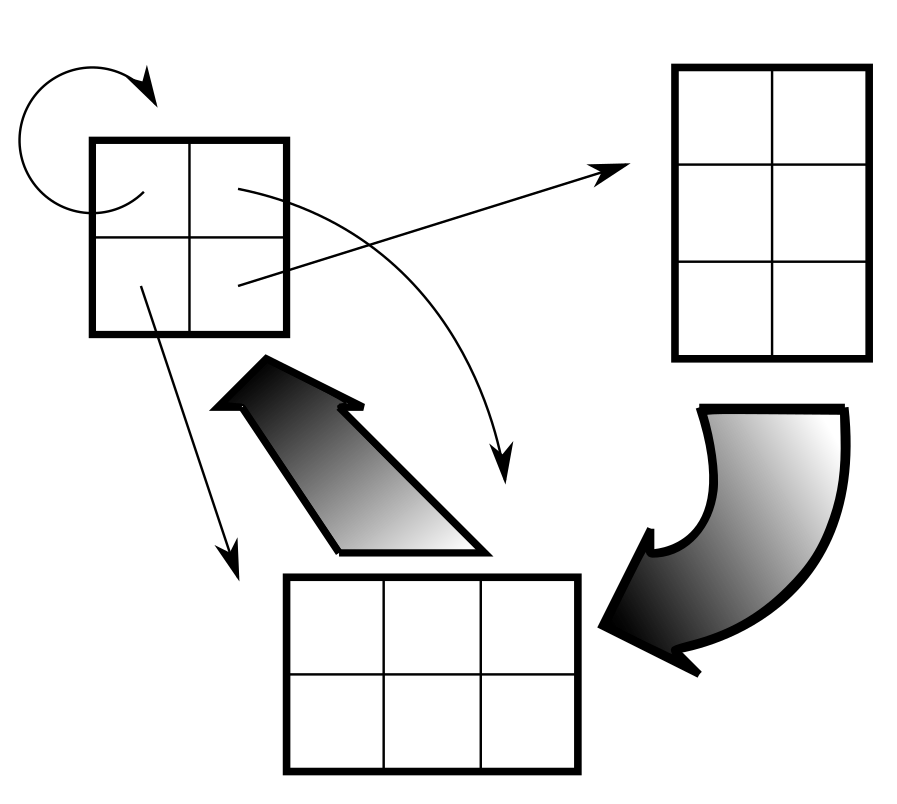
\includegraphics[width=0.25\textwidth]{img/stochastic.png}
            };
            
            \node [mybox] at (-4.5, -3) (mdp){%
                \begin{minipage}{0.40\textwidth}
                    {\color{green}Single-agent stochastic game}
                    \vspace{-0.25cm}
                    \[ |N| = 1. \]
                \end{minipage}
            };
            
            \node [mybox] at (0, -7.5) (state){%
                \begin{minipage}{\textwidth}
                    {\color{green}At every round, every player knows the
                    current state of nature $\theta \in \Theta$.} \\
                    Informally, for each player $i \in N$, there exists some
                    state $w(s_i) \in \Theta$ such that the signal $s_i$ can
                    never occur unless the current state is $w(s_i)$.
                \end{minipage}
            };
            
            \node [mybox, draw=black] at (4.5, -3.5) (std){%
                \begin{minipage}{0.60\textwidth}
                    \begin{itemize}
                        \item {\color{green}Only one possible state of
                        nature}
                        \[ |\Theta| = 1. \]
                        \item {\color{green}Players know all of each other's past
                        moves}
                        \[ S_i = \bigtimes_{j\in N-i} D_j. \]
                    \end{itemize}
                \end{minipage}
            };
            \node [inner sep=0pt] (gen-mod-img) at (7, -5.5){%
                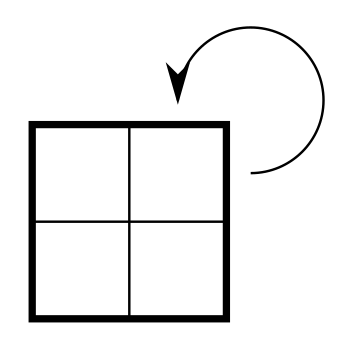
\includegraphics[width=0.20\textwidth]{img/std.png}
            };

            \node[fancytitle] at (gen-mod.north) {Stochastic Games (General Model)};
            \node[fancytitle] at (mdp.north) (mdp-title) {Markov Decision Processes};
            \node[fancytitle] at (state.north) (state-title) {Complete State Information};
            \node[fancytitle, fill=black] at (std.north) (std-title) {Standard Repeated Games};

            \draw[thick, -Latex] (gen-mod.west) -- (mdp-title.north);
            \draw[thick, -Latex] (gen-mod.south) -- (state-title.north);
            \draw[thick, -Latex] (gen-mod.east) -- (std-title.north);
        \end{tikzpicture}}
        \caption{A taxonomy of repeated game models.}
    \end{figure}
\end{frame}

\begin{frame}{Repeated game with standard information}
    \begin{block}{Definition}
        A \textit{standard repeated game} is an infinitely repeated game where a same game
        $\Gamma$ is repeated infinitely and where at each round $k$, every player knows
        all the players past moves.
    \end{block}
\end{frame}
